\documentclass[a4paper,2pt]{report}

\usepackage[a4paper, total={6in, 9in}]{geometry}
\usepackage[table,xcdraw]{xcolor}
\usepackage{pdfpages}
\usepackage{indentfirst}
\usepackage{mathtools}
\usepackage{graphicx}
\usepackage{float}
\usepackage{subfig}

\graphicspath{ {./img/} }


\setlength{\parskip}{6pt}

\begin{document}

\begin{titlepage}
    \begin{center}
        \vspace*{3cm}
 
        \LARGE
        \textbf{Instituto Superior Técnico}
        \vskip 0.4cm
 
        \Large{MEEC}
        \vskip 0.2cm

        \Large{Machine Learning}
        \vskip 3cm
        

 
        \Huge{\textbf{Lab 1}}
        \vskip 0.5cm

        \huge{\textbf{Linear Regression}}
        \vskip 0.5cm

 
        \vfill
 
        \large
        \textbf{Group 9}\\
        \vspace{0.3cm}
        Manuel Diniz, 84125\\
        Alexandre Rodrigues, 90002\\
        
        \vspace{1cm}

        \textbf{Turno:} 4ªf 11h00

    \end{center}
\end{titlepage}

\tableofcontents
\newpage

\chapter{Pre-processamento dos dados}

    \par De modo a melhor se enquadrarem ao tipo de redes neuronais a usar, os dados são alterados de forma a se obter valores para cada pixel de \(0\) a \(1\) em \textit{floating point}, ao invés dos \(0\) a \(255\) em \textit{uint8}. Valores normalizados adequam-se melhor a redes neuronais, pelo que se divide por \(255\). Para além disto converte-se a \textit{label} de cada imagem para representação \textit{one-hot}, um formato mais uma vez mais adequado para os modelos a usar.

\chapter{\textit{Multilayer perceptron}}

\chapter{\textit{Convolutional neural network}}

    \par É agora criado o modelo de uma \textit{CNN}, com a arquitetura especificada. Este modelo é treinado por um máximo de \(200\) \textit{epochs}, e programado para parar mais cedo se não existirem melhorias na aprendizagem.
    \par O \textit{calback} de \textit{early stopping} tem como objetivo evitar que o modelo fique \textit{overfit}, pelo que é muito importante que este se baseie na métrica correta para decidir quando parar a aprendizagem e restaurar os melhores pesos. A métrica a escolher é claramente \textit{val\_loss}, ou \textit{loss} de validação, isto porque é a métrica que dá uma avaliação da \textit{performance} do modelo com dados com qual este não treinou. Se fosse usado, por exemplo, a métrica \textit{loss}, que diz respeito aos dados de treino, o modelo iria tornar-se significativamente \textit{overfit}.

    \begin{figure}[H]
        \centering
        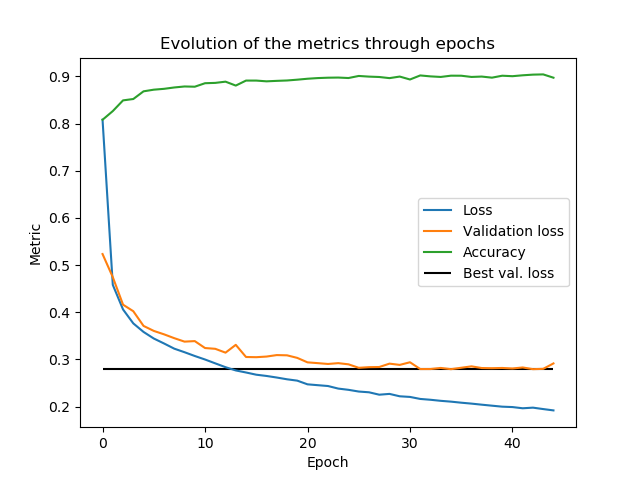
\includegraphics[width=5in]{metrics.png}
        \caption{Evolução das métricas ao longo dos \textit{epochs}}
    \end{figure}

    \par Como se pode observar, a \textit{loss} continua a diminuir muito depois da \textit{validation loss} estabilizar. Observa-se ainda uma pequena subida da \textit{validation loss} junto aos últimos \textit{epochs}, antes do \textit{early stopping} ter parado a aprendizagem. Nesta altura o modelo estava a tornar-se \textit{overfit}, melhorando a \textit{performance} nos dados de treino ao custo da nos dados de validação.

    \par A validação final com os dados de teste produz uma \textit{accuracy} de \(0.9016\), e a \textit{confusion matrix} seguinte:

    \begin{table}[H]
        \centering
        \begin{tabular}{|
        >{\columncolor[HTML]{C0C0C0}}c |c|c|c|c|c|c|c|c|c|c|}
        \hline
        Label & \cellcolor[HTML]{C0C0C0}T-shirt & \cellcolor[HTML]{C0C0C0}Trouser & \cellcolor[HTML]{C0C0C0}Pullover & \cellcolor[HTML]{C0C0C0}Dress & \cellcolor[HTML]{C0C0C0}Coat & \cellcolor[HTML]{C0C0C0}Sandal & \cellcolor[HTML]{C0C0C0}Shirt & \cellcolor[HTML]{C0C0C0}Sneaker & \cellcolor[HTML]{C0C0C0}Bag & \cellcolor[HTML]{C0C0C0}Ankle boot \\ \hline
        T-shirt & \cellcolor[HTML]{9AFF99}{\color[HTML]{333333} 870} & 0 & 24 & 25 & 2 & 1 & 71 & 0 & 7 & 0 \\ \hline
        Trouser & 1 & \cellcolor[HTML]{9AFF99}{\color[HTML]{333333} 971} & 1 & 21 & 2 & 0 & 2 & 0 & 2 & 0 \\ \hline
        Pullover & 18 & 0 & \cellcolor[HTML]{9AFF99}{\color[HTML]{333333} 868} & 7 & 37 & 0 & 67 & 0 & 3 & 0 \\ \hline
        Dress & 16 & 2 & 16 & \cellcolor[HTML]{9AFF99}{\color[HTML]{333333} 906} & 28 & 0 & 27 & 0 & 5 & 0 \\ \hline
        Coat & 1 & 1 & 53 & 19 & \cellcolor[HTML]{9AFF99}{\color[HTML]{333333} 845} & 0 & 77 & 0 & 4 & 0 \\ \hline
        Sandal & 0 & 0 & 0 & 0 & 0 & \cellcolor[HTML]{9AFF99}{\color[HTML]{333333} 971} & 0 & 21 & 0 & 8 \\ \hline
        Shirt & 153 & 0 & 68 & 21 & 56 & 0 & \cellcolor[HTML]{9AFF99}{\color[HTML]{333333} 685} & 0 & 17 & 0 \\ \hline
        Sneaker & 0 & 0 & 0 & 0 & 0 & 9 & 0 & \cellcolor[HTML]{9AFF99}{\color[HTML]{333333} 974} & 0 & 17 \\ \hline
        Bag & 3 & 1 & 8 & 4 & 4 & 2 & 7 & 5 & \cellcolor[HTML]{9AFF99}{\color[HTML]{333333} 965} & 1 \\ \hline
        Ankle boot & 1 & 0 & 0 & 0 & 0 & 4 & 0 & 34 & 0 & \cellcolor[HTML]{9AFF99}{\color[HTML]{333333} 961} \\ \hline
        \end{tabular}
    \end{table}

    \par Como se pode observar, o modelo é robusto na identificação dos objetos. O maior volume de enganos ocorre na identificação de peças de roupa semelhantes, como \textit{T-shirts} e \textit{shirts}, o que é razoável, tendo em conta que os seus formatos são parecidos.

    \par Observando agora as ativações das camadas de convolução para uma imagem exemplo, obtém-se:
    \begin{figure}[H]
        \centering
        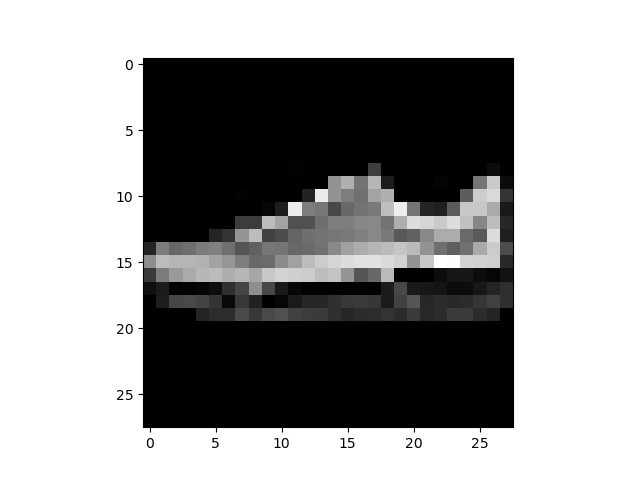
\includegraphics[width=4in]{activ_input.png}
        \caption{Imagem de teste}
    \end{figure}
    \begin{figure}[H]
        \centering
        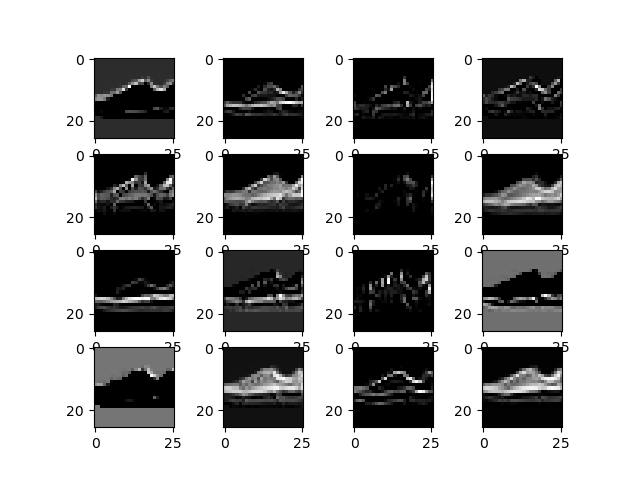
\includegraphics[width=4in]{activ_layer1.png}
        \caption{Ativação da primeira camada convolucional}
    \end{figure}

    \par Há uma certa dificuldade em tentar entender as \textit{features} que cada canal capta, pois uma rede neuronal nem sempre opera do modo que imaginamos, e há uma certa tendência de impor a nossa lógica ou forma de pensar sobre o modelo, que pode não ser correto. No entanto, parece ser possível extrapolar que o canal \(12\) (começando a contar do \(0\)) e talvez o \(11\) extraem, por exemplo, o formato geral do sapato.

    \begin{figure}[H]
        \centering
        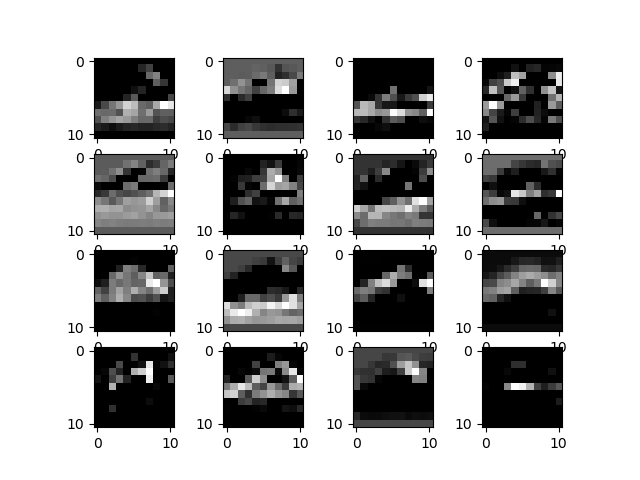
\includegraphics[width=4in]{activ_layer3.png}
        \caption{Ativação da segunda camada convolucional}
    \end{figure}

    \par A segunda convolução já não permite, através de um olho humano, entender minimamente o processo que o modelo usa, ou que \textit{features} está a identificar. Algumas ativações parecem realçar as bordas do objeto, mas é difícil dizer ao certo.


\end{document}
